\chapter{Colored Petri net-based Modeling Methodology}
\label{chapter:modeling}

\section{Problem Statement}

Consider a set of mixed-criticality component-based applications that are distributed and deployed across a cluster of embedded computing nodes. Each component has a set of interfaces that it exposes to other components and to the underlying framework. Once deployed, each component functions by executing operations observed on its component message queue. Each component is associated with a single executor thread that handles these operation requests. The nature of mixed-criticality means that these executor threads are scheduled in conjunction with a known set of highly critical system threads and other low priority \emph{best-effort} threads. Furthermore, the application threads are also subject to a temporally partitioned scheduling scheme. 

\paragraph{System Assumptions: }
\begin{enumerate}
	\item Knowledge about the component definition, component assembly, communication ports, deployment mapping, temporal partitioning etc. 
	
	\item Knowledge about the sequence of computation \emph{steps} of finite duration that are executed inside each component operation. This is dependent on the operation business-logic code written by the application developer.
	
	\item Knowledge of worst-case estimated time taken by the computational steps. There are some exceptions to this assumption e.g. blocking times on RMI calls cannot be accurately judged as these times are dependent on too many external factors.
\end{enumerate}

Using this knowledge about the system, the problem here is to ensure that the temporal behavior of the composed system meets its end-to-end timing requirements e.g. trigger-to-response times between distant sensors and actuators. Providing this guarantee implicitly requires that communicating components in a component assembly meet individual timing deadlines. Following the DREMS component model execution, a blocking I/O operation blocks a component from attending to any other requests till the operation is completed. Such blocking interaction patterns can propagate large delays to other components, especially in a highly connected system. A useful analysis result here would not only be in identifying end-to-end timing violations but also tracing delays within individual components. Tracking timing violations enables the analysis in identifying the causes for the anomalies e.g. nontrivial circular dependencies or scheduling delays. If an abstract model of the business logic of component operations is also encoded in the analysis model, then inefficient coding practices such as wasteful loops can also be marked as probable causes for deadline violations. 

Individual components need to be analyzed to identify the \emph{pure} execution times of the various computational steps in the component operations. When a set of tested components are composed together, each component's execution is affected by various factors including scheduling delays, network communication delays, blocking delays and other interaction-specific variabilities. Any timing analysis model for component-based software should account for such factors. As described in Section \ref{sec:simulation}, there are two important challenges to modeling and analyzing DRE systems: scope and abstraction level. The scope of the analysis here should be the full system of composed components. The abstraction level of the analysis must include enough detail to account for the various timing delays mentioned above while also not capturing all aspects of low-level code. A highly detailed and dynamic low-level model is necessary for simulation but not ideal for model checking and verification-based analysis due to issues like state space explosions. Also, highly composable system designs provide recombinant components that can be selected and assembled in various combinations to satisfy user requirements. In such cases, the analysis model must be efficiently capable of tackling changes in component assembly. This is a challenge when building and non-trivially generating an analysis model from a system design. Thus, efficiency, scalability and extensibility are also modeling requirements for our timing analysis.

\section{Colored Petri Net-based Analysis Model}

Petri nets have been introduced in Section \ref{sec:petri_nets}. Ordinary Petri nets have no types and no modules. Tokens are color-less dots that represent the presence or absence of some entity. The number of tokens in a place could be used to represent the quantity of some available resource. Also, ordinary Petri nets are flat structures; no hierarchy can be established to make the model more readable or concise. With Colored Petri nets (CPN), it is possible to use data types and complex data manipulations -- each token has attached a data value, called the token \emph{color}. This token color can be investigaed and modified by the occurring transitions. With CPN, it is also possible to make hierarchical descriptions i.e. a large model can be obtained by combining a set of submodels with well-defined interfaces between submodels and well-defined semantics of the combined model. Furthermore, each submodel can be reused. 

One of the primary reasons for choosing Colored Petri Nets over other high-level Petri Nets such as Timed Petri Nets or other modeling paradigms like Timed Automata is because of the powerful modeling concepts made available by token colors. Each \emph{colored token} can be a heterogeneous data structure such as a \emph{record} that can contain an arbitrary number of fields. This enables modeling within a single \emph{color-set} (C-style \texttt{struct}) system properties such as temporal partitioning, component interaction patterns, and even distributed deployment. The token colors can be inspected, modified, and manipulated by the occurring transitions and the arc bindings. Component properties such as thread priority, port connections and real-time requirements can be easily encoded into a single colored token, making the model considerably concise. 

The CPN analysis model, as modeled in CPN Tools \cite{CPNTools}, is shown in Figure \ref{fig:hlcpn}. \emph{Places}, shown as ovals, in this model contain colored (typed) tokens that represent the state of interest for analysis e.g. \emph{Clocks} place holds tokens of type \emph{clocks} maintaining information regarding the state of the clock values and temporal partition schedule on all computing nodes. \emph{Transitions}, shown as rectangular boxes, are responsible for executing this model, progressing the state of the modeled system and transferring tokens between places. \emph{Arcs}, between transitions and places dictate the token flow and data structure manipulations. All arcs contain emph{inscriptions}, which are essentially function calls, written in Standard ML, that manipulate token structures e.g. arc inscriptions in the arc from the transition \emph{Timer\_Expiry} to the place \emph{Timers}, manipulate all timer tokens by updating the timer expiry offsets. 

\begin{figure}[h]
	\centering
	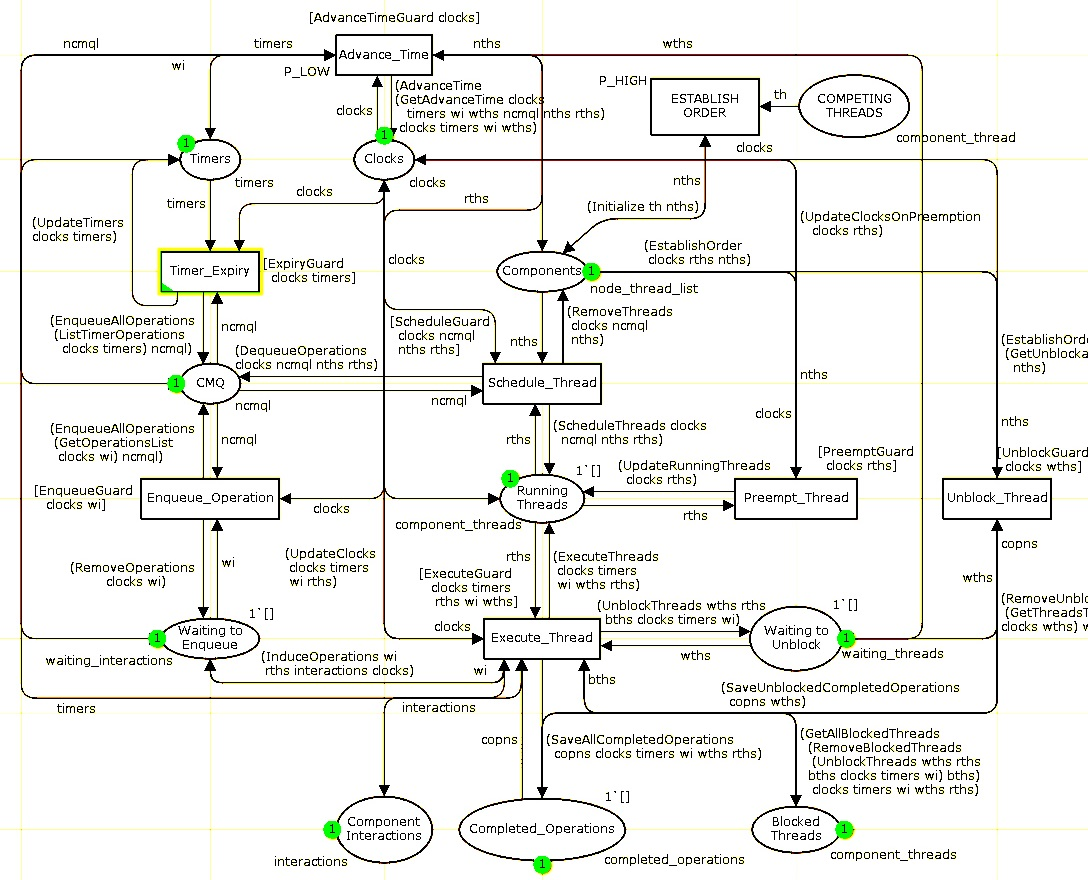
\includegraphics[width=\textwidth]{hlcpn_cropped}
	\caption{Colored Petri Net Analysis Model}
	\label{fig:hlcpn}
\end{figure}

From the design model of the system, we generate the initial CPN tokens that are injected into places in this analysis model. Using the in-built state space analysis engine, we analyze the state space of the parameterized model to compute useful system properties e.g. processor utilization, execution time plots, deadline violations etc. The modeling concepts in Figure \ref{fig:hlcpn} can be divided and categorized based on system-level concepts being analyzed. Figure \ref{fig:hlcpn_structure} shows the organizational structure of this CPN. Below, we describe each of these structural divisions in detail. 

\begin{figure}[h]
	\centering
	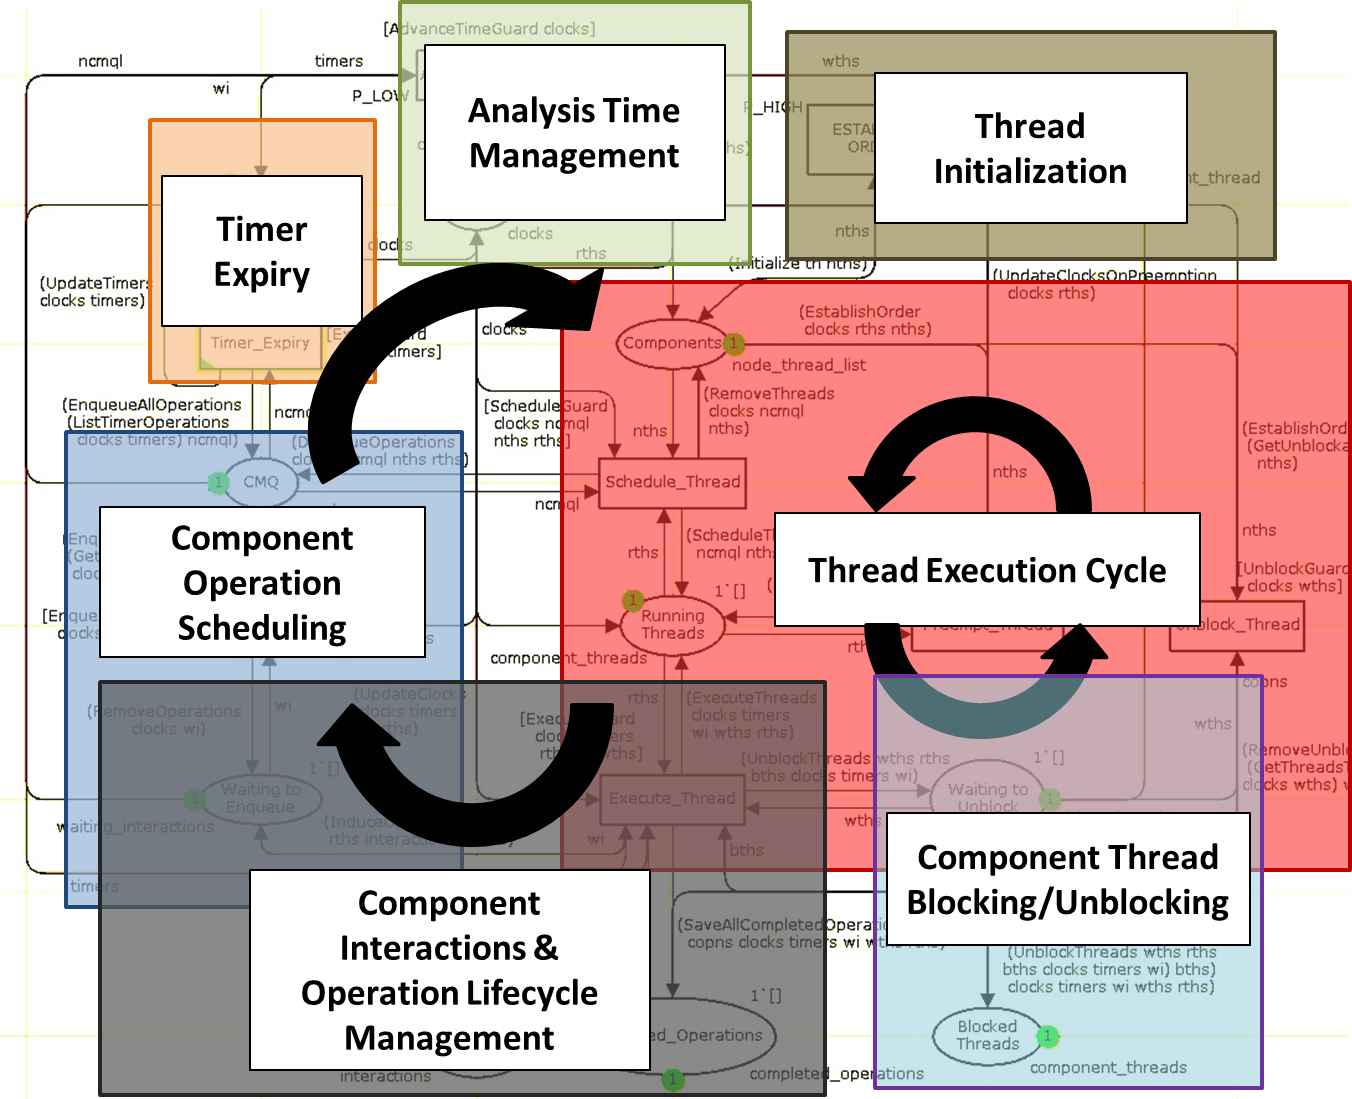
\includegraphics[width=\textwidth]{hlcpn_structure}
	\caption{Analysis Model - Structural Aspects}
	\label{fig:hlcpn_structure}
\end{figure}

\subsection{Model of Time}
\label{sec:model_of_time}

Appropriate choice for temporal resolution is a necessary first step in order to model and analyze threads running on a processor. The OS scheduler enforces temporal partitioning and uses a priority-based scheme for threads active within a temporal partition. If multiple threads have the same priority, a round-robin (RR) scheduling is used. In order to observe and analyze this behavior, we have chosen the temporal resolution to be 100 us; a fraction of 1 clock tick of the OS scheduling quantum. In Section \ref{handling_time}, we describe the disadvantages of managing time as a fixed-step increasing variable and describe our solutions that significantly improve the generated state space and the efficiency of the analysis. 

%\subsubsection{Dynamic Time Progression:}
%Although the time resolution at the start of the analysis is chosen to be 1 ms, this is not a constant throughout the execution of the analysis model. If it were, then \emph{S} seconds of activity will generate a state space of size: $SS_{size} = \sum\limits_{i=1}^{S*1000} TF_{t_i}$
%where $TF_{t_i}$ is the number of state-changing CPN transition firings between $t_i$ and $t_{i+1}$. This large state space includes intervals of time where there is no thread activity to analyze either due to lack of operation requests, lack of ready threads for scheduling, or due to temporal partitioning. During such idle periods, the analysis engine dynamically increases the time-step size and progresses time either to (1) the next node-specific clock tick, (2) the next global timer expiry offset, (3) the next operation enqueue time stamp, (4) thread lifecycle change or (5) the next node-specific temporal partition (whichever is earliest and most relevant). This ensures that the generated state space tree is devoid of nodes where there is no thread activity. Such dynamic control of time using global variables during analysis is also one of the advantages of using Colored Petri nets. 

\subsection{Modeling Temporal Partitioning}
The place \emph{Clocks} in Figure \ref{fig:hlcpn} holds the state of the node-specific global clocks. The temporal partition schedule modeled by these clocks enforces a constraint: component operations can be scheduled and component threads can be run only when their parent partition is active. Each clock token \emph{NC} is modeled as a 3-tuple:

\vspace{-0.15in}
\begin{equation}
\label{eq:NC}
NC = \ < Node_{NC}, \ Value_{NC}, \ TPS_{Node_{NC}} >
\end{equation}

where, $Node_{NC}$ is the name of the computing node, $Value_{NC}$ is an integer representing the value of the global clock and $TPS_{Node_{NC}}$ is the temporal partition schedule on $Node_{NC}$. Each \emph{TPS} is an ordered list of temporal partitions.

\vspace{-0.15in}
\begin{equation}
\label{eq:TP}
TP = \ < Name_{TP}, \ Prd_{TP}, \ Dur_{TP}, \ Off_{TP}, \ Exec_{TP} >
\end{equation}

Each partition $TP$ (Eq. \ref{eq:TP}) is modeled as a record color-set consisting of a name $Name_{TP}$, a period $Prd_{TP}$, a duration $Dur_{TP}$, an offset $Off_{TP}$ and the state variable  $Exec_{TP}$. %Aggregate of such partitions can fully describe a partition schedule. Complete partition schedules are maintained per computing node.

\subsection{Modeling Component Thread Behavior}

Figure \ref{fig:Thread_Execution} presents a snippet of our CPN, modeling the thread execution cycle. The place \emph{Components} holds tokens that keep track of all the ready threads in each computing node. Each component thread $CT$ is a record characterized by:

\begin{equation}
\label{eq:CT}
CT = \ <ID_{CT}, \ Prio_{CT}, \ O_{CT}>
\end{equation}

where $ID_{CT}$ constitutes the concatenation of strings required to identify a component thread in CPN (i.e. component name, node name and partition). Every thread is characterized by a priority ($Prio_{CT}$) which is used by the OS scheduler to schedule the thread. 
%The DREMS OS uses a fixed-priority preemptive scheduling scheme (constrained by temporal partitioning) to schedule component threads. %If multiple threads belonging to the same temporal partition are ready, the highest priority thread is always chosen for execution. If there is more than one candidate thread, one is chosen at random, followed thereafter by a Round-Robin scheduling scheme. 

\begin{figure}[htb]
	\centering
	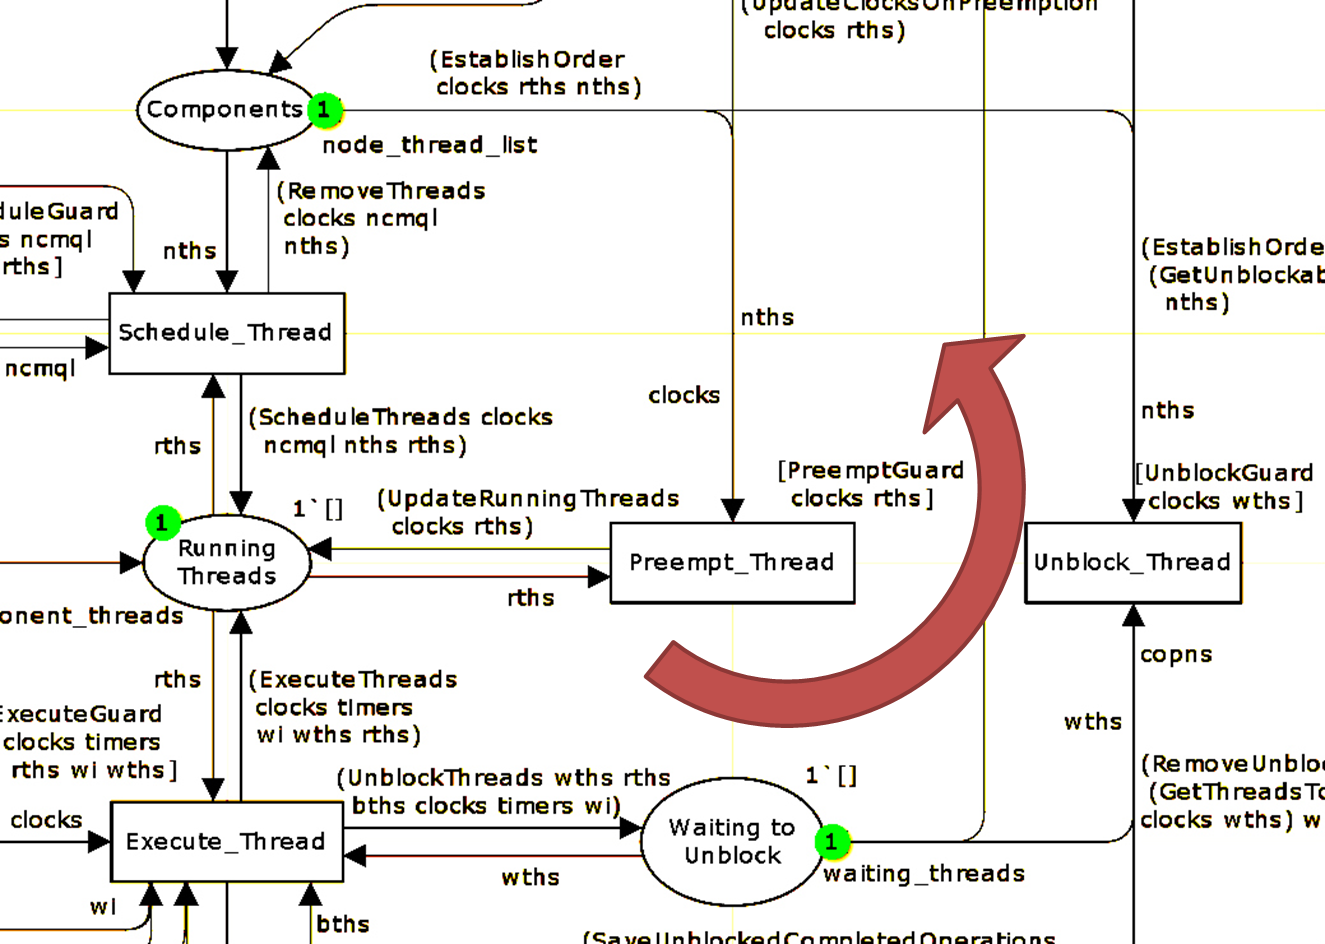
\includegraphics[width=\textwidth]{source-thread_execution_cycle}
	\caption{Component Thread Execution Cycle}
	\label{fig:Thread_Execution}
\end{figure}

If the highest priority (OS schedulable) thread is not already servicing an operation request, the next ready operation from the message queue is dequeued and scheduled for execution (represented by $O_{CT}$). Depending on the component scheduler, this operation may be the highest priority, or may have the earliest deadline or may be the oldest request. The scheduled thread token is placed in \emph{Running Threads}. %The guard on \emph{Schedule Thread} ensures that the highest priority thread in the currently running partition is scheduled first. 

When a thread token is marked as running, the model checks to see if the thread execution has any effect on itself or on other threads. These state changes are updated using the transition \emph{Execute\_Thread} which also handles time progression. Keeping track of $Value_{NC}$, the thread is preempted at each clock tick. This transition loop i.e. \emph{Schedule\_Thread -> Execute\_Thread -> Preempt/Unblock\_Thread -> Schedule\_Thread ...} cycle repeats forever, as long as there are no system-wide deadlocks and some upper limit on the clock values isn't reached.

\subsection{Modeling Component Operations}
\label{sec:Modeling_Component_Operations}
Every operation request \emph{O} made on a component \emph{$C_x$} is modeled as a Standard ML \emph{record} of the 4-tuple:

\begin{equation}
O(C_x) = \ < ID_O, \ Prio_O, \ Dl_O, \  Steps_O >
\end{equation}

where, $ID_O$ is a unique concatenation of strings that help identify and locate this operation in the system (consisting of the name of the operation, the component, the computing node, and the temporal partition). Assuming a PFIFO operation scheduling scheme, the operation's priority ($Prio_O$) is used by the analysis engine to enqueue this operation request on the message queue of $C_x$. The analysis model also supports FIFO and EDF schemes. The completion of this enqueue implies that this operation has essentially been \emph{scheduled} for execution. Once enqueued, if this operation does not execute and complete before its fixed deadline ($Dl_O$), its real-time requirements are violated. 

Once an operation request is dequeued, the execution of the operation is modeled as a transition system that runs through a sequence of \emph{steps} dictating its behavior. Any of these underlying steps can have a state-changing effect on the thread executing this operation e.g. interactions with I/O devices on the component-level could block the executing thread (for a non-deterministic amount of time) on the OS-level. Therefore, every component operation has a unique list of steps ($Steps_O$) that represent the sequence of local or remote interactions undertaken by the operation. Each of the \emph{m} steps in $Steps_O$ is a 4-tuple:

\begin{equation}
s_i = \ <Port, \ Unblk_{s_i}, \ Dur_t, \ Exec_t>
\end{equation}

where $1 \le i \le m$. \emph{Port} is a \emph{record} representing the exact communication port used by the operation during $s_i$. $Unblk_{s_i}$ is a list of component threads that are unblocked when $s_i$ completes. This list is used, e.g., when the completion of a synchronous remote method invocation on the server side is expected to unblock the client thread that made the invocation. Finally, temporal behavior of $s_i$ is captured using the last two integer fields: \emph{$Dur_t$} is the worst-case estimate of the time taken for $s_i$ to complete and $Exec_t$ is the relative time of the execution of $s_i$, with $0 \le Exec_t \le Dur_t$.

Consider the simple RMI application show in Figure \ref{fig:rmi_application}. The application has two components, a client and a server. The client component is associated with a periodic timer that triggers a sequence of interactions between the two components. When the client timer expires, a timer operation is enqueued on the client's operation queue. When scheduled, the client executor thread executes this operation, which makes an RMI call to the server component. Once the query is made, the client thread is effectively blocked till a response is received. The server thread that produces this response may not be scheduled immediately due to the constraints of temporal partition scheduling and other thread scheduling delays. Once the RMI operation is completed on the server, the client thread is unblocked. 

\begin{figure}[ht]
	\centering
	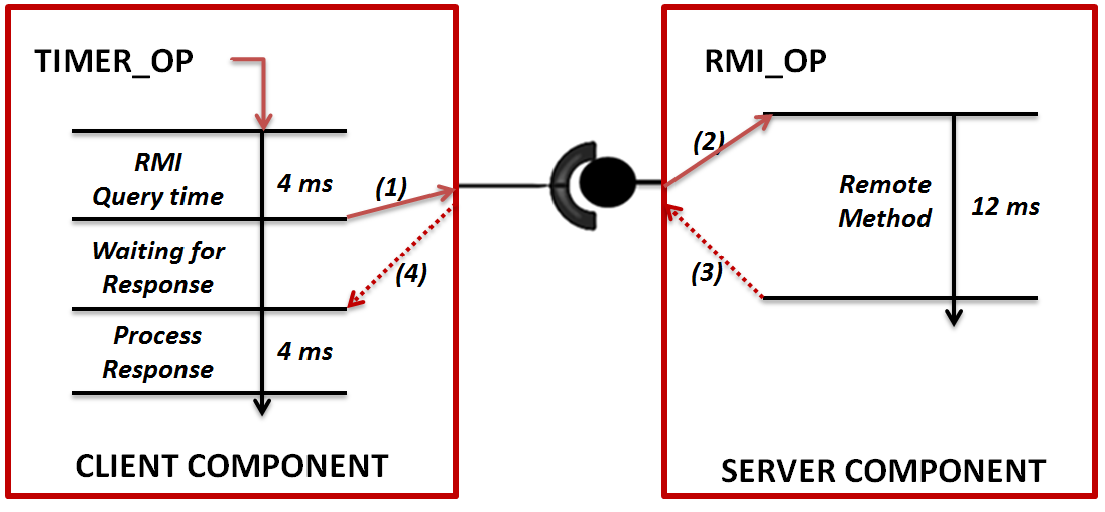
\includegraphics[width=\textwidth]{rmi_application}
	\caption{RMI Application}
	\label{fig:rmi_application}
\end{figure}

In the above example, the duration of time for which the client is blocked, is dependent on, among several factors, what happens inside the remote method on the server. This remote method could either simply take up CPU time, interact with the underlying framework or interact with other components in the application. To capture such interaction patterns, the \emph{step} color-set is defined in CPN. In this example, two \emph{operation} tokens are required to describe the operations handled by the components: a client side timer operation and a server side RMI operation. A sample client timer operation is shown in Figure \ref{fig:cpn_rmi_app_timer_token}.

\begin{figure}[ht]
	\centering
	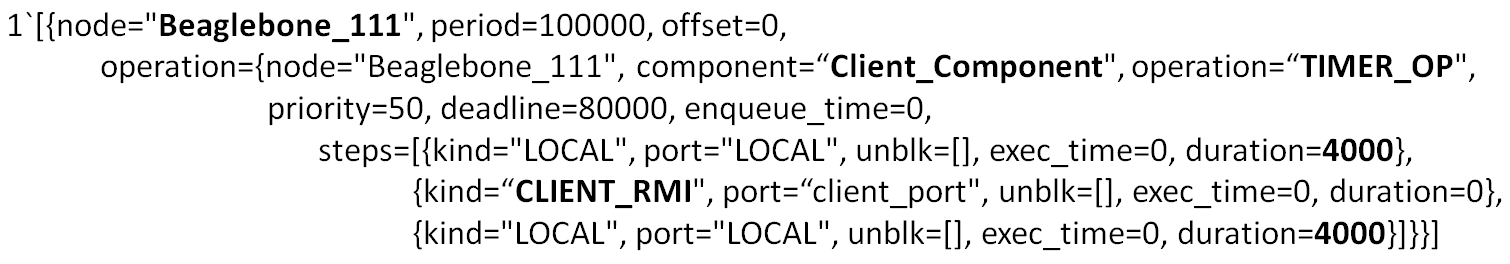
\includegraphics[width=\textwidth]{cpn_rmi_app_timer_token}
	\caption{RMI Application - Client Timer Operation}
	\label{fig:cpn_rmi_app_timer_token}
\end{figure}

This timer operation runs on the client component with a priority of 50, and a deadline of 80 ms. The business logic of this operation consists of a single RMI call that takes 4 ms to send out the query after which it blocks the executing client thread. After the client thread runs for time \emph{t = q\_t}, the client thread is moved to a blocked state and an RMI operation is induced on the server side. The client side thread remains blocked until the server thread completes executing the remote method. Once the server thread completes execution, it sends the response of the RMI back to the client. The model takes note of how long the client has been blocked by using the time stamp at which it receives a response. The client thread runs for an additional 4 ms to process this response before it marks completion. The token for the server RMI operation is shown in Figure \ref{fig:cpn_rmi_app_server_token}. Note that all time measurements in this token are in micro-seconds i.e. a step duration of 4000 implies 4 ms of activity. The requested RMI operation is run on the server component with a priority of 50 and a deadline of 15 ms. The deadline of this operation cannot be worse than the deadline of the client side operation that initiated the interaction. If this operation delays past 80 ms, a client side deadline violation is realized as the client thread is blocking for longer than expected. 

\begin{figure}[ht]
	\centering
	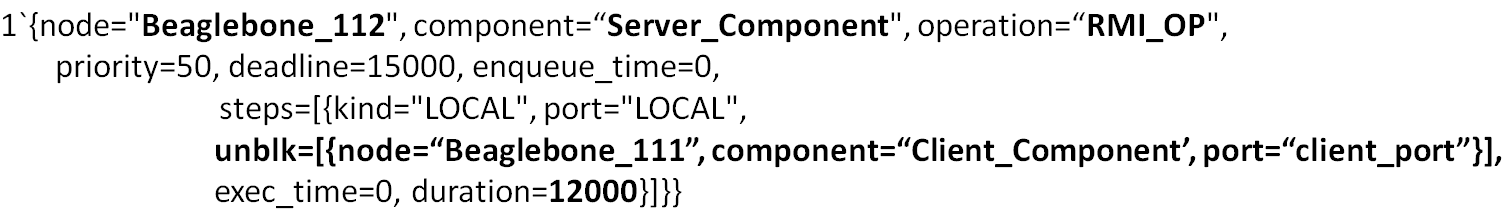
\includegraphics[width=\textwidth]{cpn_rmi_app_server_token}
	\caption{RMI Application - Server Operation}
	\label{fig:cpn_rmi_app_server_token}
\end{figure}


\subsection{Modeling Component Interactions}

In our earlier RMI example, the client is periodically triggered by a timer to make a remote method call to the server. When the client executes an instance of this timer-triggered operation, a related operation request is enqueued on the server's message queue. In reality, this is handled by the underlying middleware. Since the details of this framework are not modeled, the server-side request is captured as an \emph{induced operation} that manifests as a consequence of the client-side activity. Tokens that represent such design-specific interactions are maintained in the place \emph{Component Interactions} (Figures \ref{fig:hlcpn},\ref{fig:cpn_iop}) and modeled as shown in equation \ref{eq:component_interactions}. The interaction \emph{Int} observed when a component $C_x$ queries another component $C_y$ is modeled as the 3-tuple:

\begin{equation}
\label{eq:component_interactions}
Int(C_x, C_y) = \ < Node_{C_x}, \ Port_{C_x}, \ O(C_y)>
\end{equation}

When an operational \emph{step} in component $C_x$ uses port $Port_{C_x}$ to invoke an operation on component $C_y$, the request $O_{C_y}$ is enqueued on the message queue of $C_y$. 

 \begin{figure}[ht]
 	\centering
 	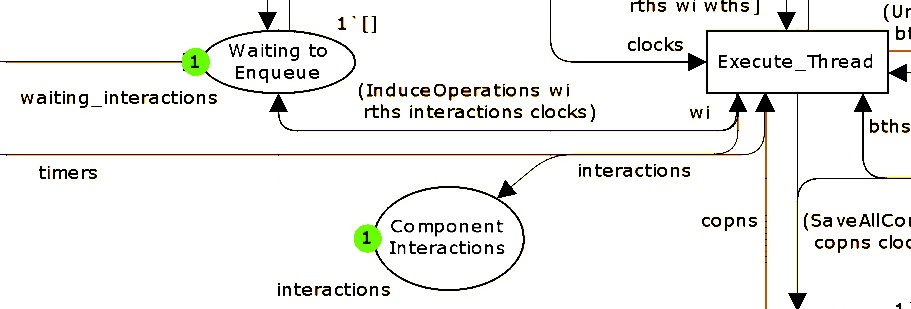
\includegraphics[width=\textwidth]{component_interactions}
 	\caption{Operation Induction}
 	\label{fig:cpn_iop}
 \end{figure} 
 
Every \emph{interaction} token contains an interaction port and an operation. The transition \emph{Execute\_Thread} observes the activity on the currently running thread. When executing the model, if a particular step executed by a component thread would, on completion, request the services of another component, a token is placed on the \emph{Waiting to Enqueue} place. So, once the client thread pushes out an RMI query, an operation needs to be induced on the server queue. So an \emph{interaction} token for this communication is constructed. The model waits for the RMI call on the client side to complete, at which point it places the operation \emph{i\_op} on the server message queue. This induction is represented in Figure \ref{fig:cpn_rmi_app_iop}. 

 \begin{figure}[h]
 	\centering
 	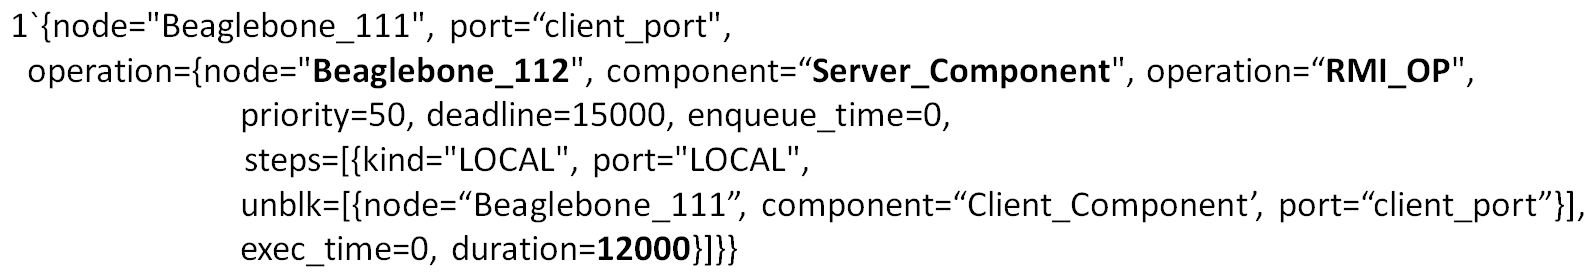
\includegraphics[width=\textwidth]{cpn_rmi_app_iop}
 	\caption{Operation Induction Token}
 	\label{fig:cpn_rmi_app_iop}
 \end{figure}

\subsection{Modeling Timers}

DREMS components are inactive initially; once deployed, a component executor thread is not eligible to run until there is a related operation request in the component's message queue. To start a sequence of component interactions, periodic or sporadic timers can be used to trigger a component operation. In CPN, each timer $TMR$ is held in the place \emph{Timers} and represented as shown in Eq. \ref{eq:TMR}. Timers are characterized by a period ($Prd_{TMR}$) and an offset ($Off_{TMR}$). Every timer triggers a component using the operation request $O_{TMR}$.

\begin{equation}
\label{eq:TMR}
TMR = \ < Prd_{TMR}, \ Off_{TMR}, \ O_{TMR}>
\end{equation} 

When the component's timer expires, a timer callback operation is placed on the component message queue. When the component executor thread is picked by the OS scheduler, this operation is dequeued and the timer callback is executed. In CPN, timer operations are modeled as shown in Figure \ref{fig:cpn_timers}. 

\begin{figure}[ht]
	\centering
	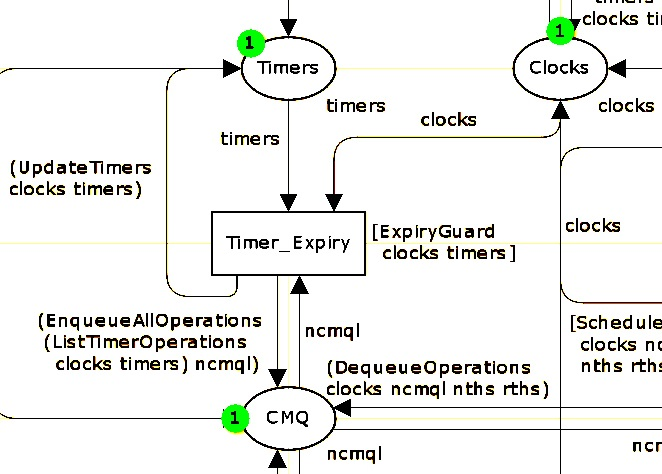
\includegraphics[width=\textwidth]{timers}
	\caption{Timer Operations}
	\label{fig:cpn_timers}
\end{figure}

All component timers are expressed as separate tokens and initialized in the \emph{Timers} place. It is important to note that the enqueue operation does not happen until the appropriate partition is active. This is because the component-specific thread responsible for enqueueing (or dequeuing) incoming operations is also affected by temporal partitioning. 

\section{Modeling Component Operation Business Logic}
\label{sec:BL_Model}

\subsection{Problem Statement}

Consider a set of component-based applications deployed on distributed hardware. Each application consists of groups of components that interact with each other and also with the external environment e.g. I/O devices, other applications, underlying middleware etc. Each component exposes a set of interfaces through which external entities can request \emph{operations}. As mentioned earlier, an operation is an abstraction for the different tasks undertaken by a component. These operations are exposed through ports and can be requested by other components. When an operation is requested, the request is placed in the component's message queue and eventually serviced. When ready, the business logic of the operation i.e. a local callback is executed. This piece of code represents the brains of the operation. The goal here is to be able to model this business logic, for every component operation, effectively as part of the design model, including temporal estimates such as worst-case execution times for individual code blocks, so that the model can be translated into appropriate data structures in our CPN analysis model.

\subsection{Challenges}

The execution of component operations service the various periodic or aperiodic interaction requests coming from either a timer or other connected (possibly distributed) components. Each operation is written by an application developer as a sequence of execution steps. Each step could execute a unique set of activities, e.g. perform a local calculation or a library call, initiate an interaction with another component, process a response from external entities, and it can have data-dependent, possibly looping control flow, etc. The behavior derived by the combination of these steps contribute to the worst-case execution of the component operation. The behavior may include non-deterministic delays due to component interactions while being constrained by the temporally partitioned scheduling scheme and hardware resources. The challenge here is to identify a metamodel grammar that would represent the potentially dynamic behavior realized in a component operation. The modeling aspects emerging from this challenge will have to propagate to any timing analysis model that studies the system. This is true because any non-deterministic delays such as blocking times need to be accounted for when analyzing the temporal behavior.

\subsection{Outline of Solution}
The business-logic model of a component operation requires to be completely integrated into our CPN modeling methodology. This means that the model, however complex, needs to be translated into some token data structure in CPN. This is our primary constraint. The CPN analysis model needs to know how an operation is structured i.e. what are the sequential steps in the code, along with WCET on each step. Lastly, since the CPN model does not model or simulate component data management, data-dependent conditional statements in the business-logic model were avoided or abstracted away. Following these rules, we designed a metamodel for the component operation business logic. Each component operation model is then attached to a component port or timer in the main design model and enriches the model with refined details about the workings of the operation. In summary, this model is capable of representing several types of code blocks including local function calls, remote procedure calls, outgoing port-to-port interactions, incoming port-response processing, and bounded loops.

The execution of component operations service the various periodic or aperiodic interaction requests coming from either a timer or other connected (possibly distributed) components. Each operation is written by an application developer as a sequence of execution \emph{steps}. Each step could execute a unique set of activities, e.g. perform a local calculation or a library call, initiate an interaction with another component, process a response from external entities, and it can have data-dependent, possibly looping control flow, etc. The behavior derived by the combination of these steps contribute to the worst-case execution of the component operation. The behavior may include non-deterministic delays due to component interactions while being constrained by the  temporally partitioned scheduling scheme and hardware resources. This section briefly describes the various aspects of this behavior specification that are general enough to be applicable to a range of component-based systems.

\begin{figure}[ht]
	\centering
	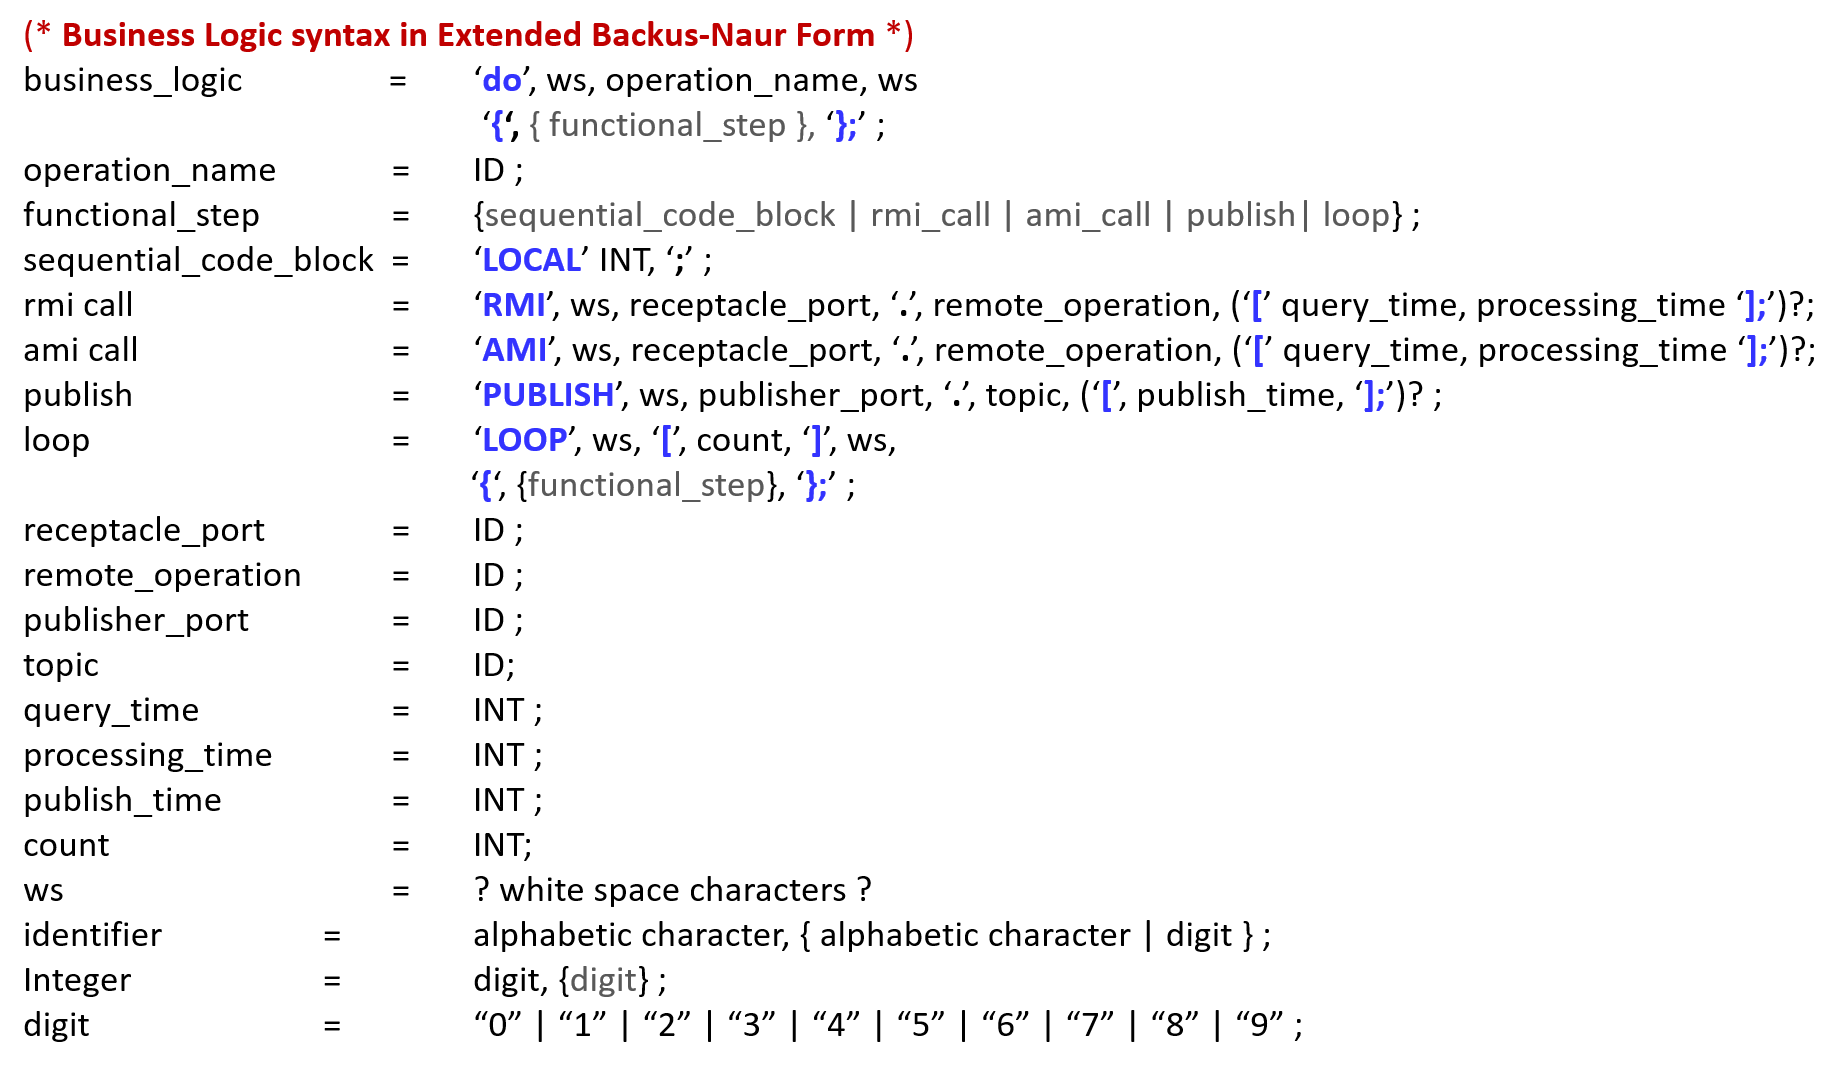
\includegraphics[width=\textwidth]{./img/BL-EBNF}
	\caption{Modeling the Business Logic of Component Operations}
	\label{fig:ebnf}
\end{figure}

Figure \ref{fig:ebnf} shows the Extended Backus-Naur form representation of the grammar \cite{SEUS} used for modeling the business logic of component operations. The symbol \emph{ID} represents identifiers, a unique grouping of alphanumeric characters, and the symbol \emph{INT} represents positive integers. Each operation is characterized by a unique name, a priority, and a deadline. The priority is an integer used to resolve scheduling conflicts between operations \emph{provided} by the same component when multiple messages from other entities are received. The arbitration is handled by the component-level scheduler. The deadline of the operation is the worst-case time that can elapse after the operation is marked as \emph{ready} and the completion of the operation. The business logic of every component operation is modeled as a sequence of steps, each with an assigned worst-case execution time. We broadly classify these steps into (1) blocks of sequential code, (2) peer-to-peer synchronous and asynchronous remote calls, (3) anonymous publish/subscribe distribution service calls, (4) blocking and non-blocking I/O interactions and (5) bounded control loops. 

Notice the integration of timing properties such as worst-case function call times e.g. RMI calls  (\emph{query\_time}), worst-case argument processing times (\emph{processing\_time}) and DDS publish times (\emph{publish\_time}). If these expected delays are set to zero, the analysis will execute these interactions in a single synchronous step taking no time. However, in reality these steps still take a non-zero amount of time to execute. Therefore, if such metrics are not known then these values can be set to zero and an overall worst-case execution time can be set per operation. This is the maximum amount of time that can elapse after the component operation has begun to execute. This time will include all component interactions and network delays that affect the operation's execution. 

\begin{figure}[ht]
	\centering
	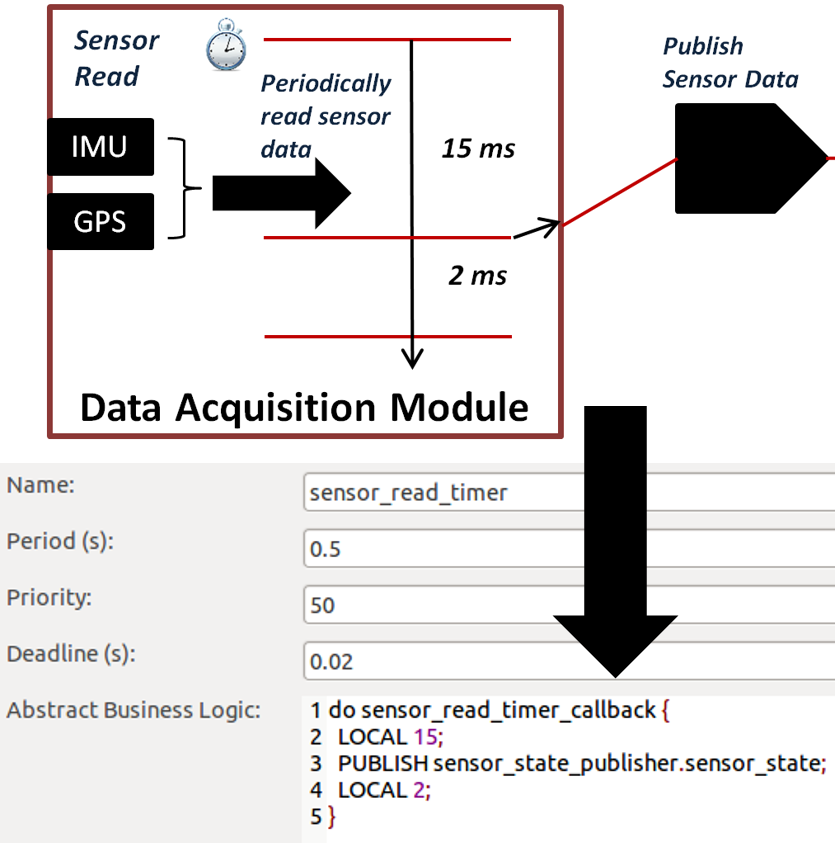
\includegraphics[width=0.8\textwidth]{./img/abstract_business_logic}
	\caption{Sample Business Logic Model}
	\label{fig:sblm}
\end{figure}

Figure \ref{fig:sblm} shows a sample business logic model conforming to this grammar. The Data Acquisition Module is a periodically triggered I/O component i.e. this component receives a stream of sensor information from various sensor devices e.g. inertial measurement units (IMU) and GPS modules. This component packages this information and publishes sensor state as a message to all subscribers e.g. controller components. Figure \ref{fig:sblm} shows the translation from the conceptual understanding of the workings of this component operation to the abstract business logic model that is then translated into CPN tokens (Figure \ref{fig:blte}), as described in Section \ref{sec:Modeling_Component_Operations}. 

\begin{figure}[ht]
	\centering
	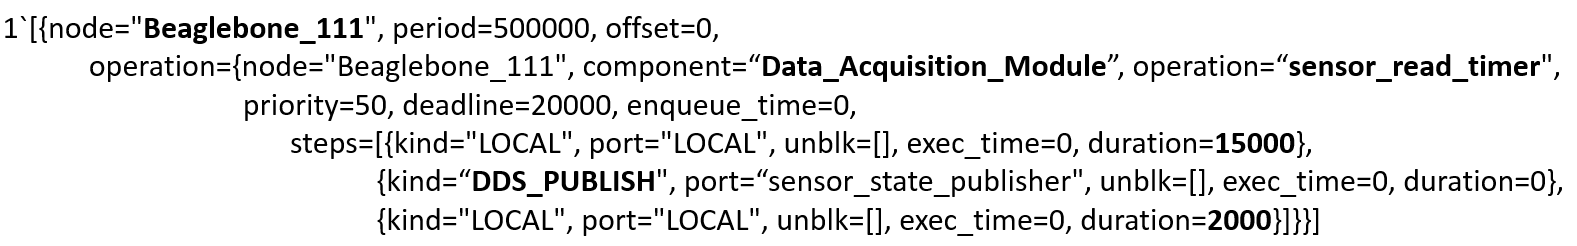
\includegraphics[width=\textwidth]{./img/cpn_business_logic_token_example}
	\caption{CPN Business Logic Representation}
	\label{fig:blte}
\end{figure}